%This work is licensed under the Creative Commons License Attribution 4.0 International (CC-BY 4.0)
%https://creativecommons.org/licenses/by/4.0/legalcode
\documentclass[rgb]{standalone}
\usepackage{pgfplots}
\usepgfplotslibrary{patchplots,colorbrewer}
\pgfplotsset{colormap/Greys-7}
\definecolor{myblue}{hsb}{0.5833, 1, 0.8}
\begin{document}
	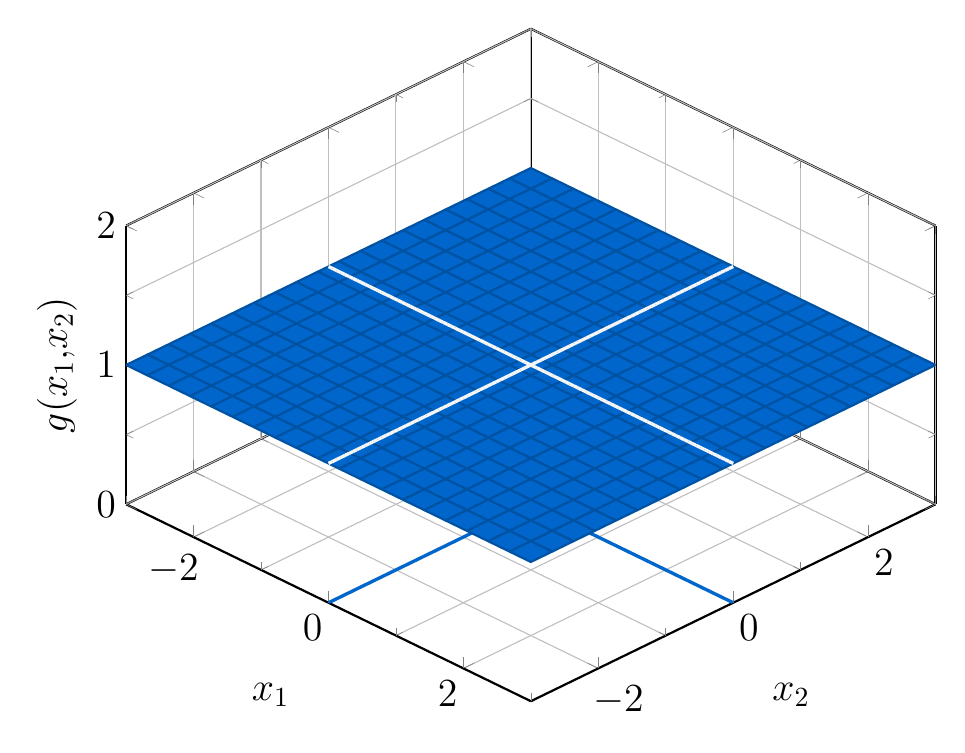
\begin{tikzpicture}[font=\Large]
		\begin{axis}[scale=1.5,thick,grid=both, minor tick num =1,view={45}{45},
			xmin=-3, xmax=3, ymin=-3,ymax=3, zmin=0, zmax=2, 
			ztick={0,1,2}, 
			mesh/interior colormap=
			{interior}{color=(myblue) color=(myblue)},
			xlabel=$x_1$, ylabel=$x_2$, zlabel=$g(x_1 {,} x_2)$]
		\draw[very thick, myblue] (axis cs:-3,0,0) -- (axis cs:3,0,0) ;
		\draw[very thick, myblue] (axis cs:0,-3,0) -- (axis cs:0,3,0) ;		
		\addplot3[surf, patch, domain=-3:3, y domain=-3:3,
			samples=20] {1};
			\addplot3 [smooth, patch, very thick, domain=-3:3, samples = 100, samples y=0] ( {x}, {0}, {1});	
			\addplot3 [smooth, patch, very thick, domain=-3:3, samples = 100, samples y=0] ( {0}, {x}, {1});
		\end{axis}
	\end{tikzpicture}
\end{document}